\chapter{Marco Teórico}\label{sec:Marco_Teorico}
\thispagestyle{empty}
\newcommand{\subsubsubsection}[1]{\paragraph{#1}\mbox{}\\}
\setcounter{secnumdepth}{4}
\setcounter{tocdepth}{4}

\newcommand{\subsubsubsubsection}[1]{\paragraph{#1}\mbox{}\\}
\setcounter{secnumdepth}{5}
\setcounter{tocdepth}{5}

\begingroup
\rightskip0.5cm
\small

\endgroup

\par En el capítulo a continuación se describirá los conceptos y la terminología necesaria para realizar acabo el proyecto de grado.
\par cita \cite{}
\section{Red eléctrica inteligente}
  \par Al pasar de los años el sistema eléctrico ha evolucionado con vistas a mejorar la eficiencia energética, la confiabilidad y seguridad de las redes eléctricas. Actualmente ese sistema evolucionado los conocemos como una red eléctrica inteligente o por su traducción en ingles \textit{Smart Grid}. Sin embargo, a pesar de que este nuevo sistema se encuentre en desarrollo desde hace algunos años aun no se ha logrado formalizar una definición concreta y universal. En la búsqueda de establecer una definición global, instituciones como las siguientes han propuesto las siguientes:

  \par El Departamento de Energía de Estados Unidos (REFERENCIA):
  \par \textit{A smart grid uses digital technology to improve reliability, security, and efficiency (both economic and energy) of the electric system from large generation, through the delivery systems to electricity consumers and a growing number of distributed-generation and storage resources.}

  \par La Comisión Electrotécnica Internacional IEC (REFERENCIA):
  \par \textit{The Smart Grid is integrating the electrical and information technologies in between any point of generation and any point of consumption}

  \par Interpretando las definiciones anteriores podemos definir las redes eléctricas inteligentes como un sistema que permitira el manejo de la energía eléctrica y la integración de las energias de renovables de una manera mas eficiente, mediante instrumentos que permiten controlar la distruibucion de la enérgia, la obtencion del estado de la red y la comunicacion bidireccional entre estos dispositivos y la estación eléctrica.

  \par Actualmente la Comisión Electrotécnica Internacional conocida por sus siglas en ingles como IEC se encuentra desarrollando los estandares internacionales que regirán las Redes Eléctricas Inteligentes. En la figura LABEL se encuentra un modelo de como se debe considerar una Smart Grid, modelo que se establecio debido al proceso de estandarización.

  \begin{figure}[H]
    \centering
    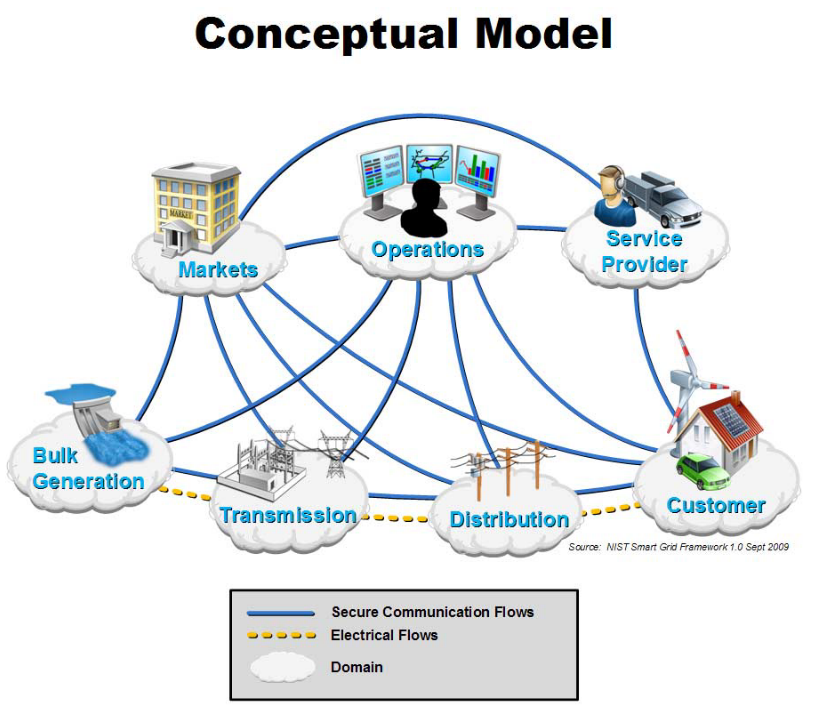
\includegraphics[width=0.8\textwidth]{../Imagenes/modelo_SG.png}
    \caption{Modelo conceptual de la red eléctrica inteligente REFERENCIA}
    \label{fig:model_SG}
  \end{figure}


\section{Medidores inteligentes}
  \par

  \par Cada dia los avances tecnológicos han hecho evolucionar los medidores de consumo eléctrico, agregando nuevas funciones y mejorando la precisión de las mediciones. En la figura LABEL se presenta la evolución que han presentado los medidores y las distintas funciones agregadas.

  \begin{figure}[H]
    \centering
    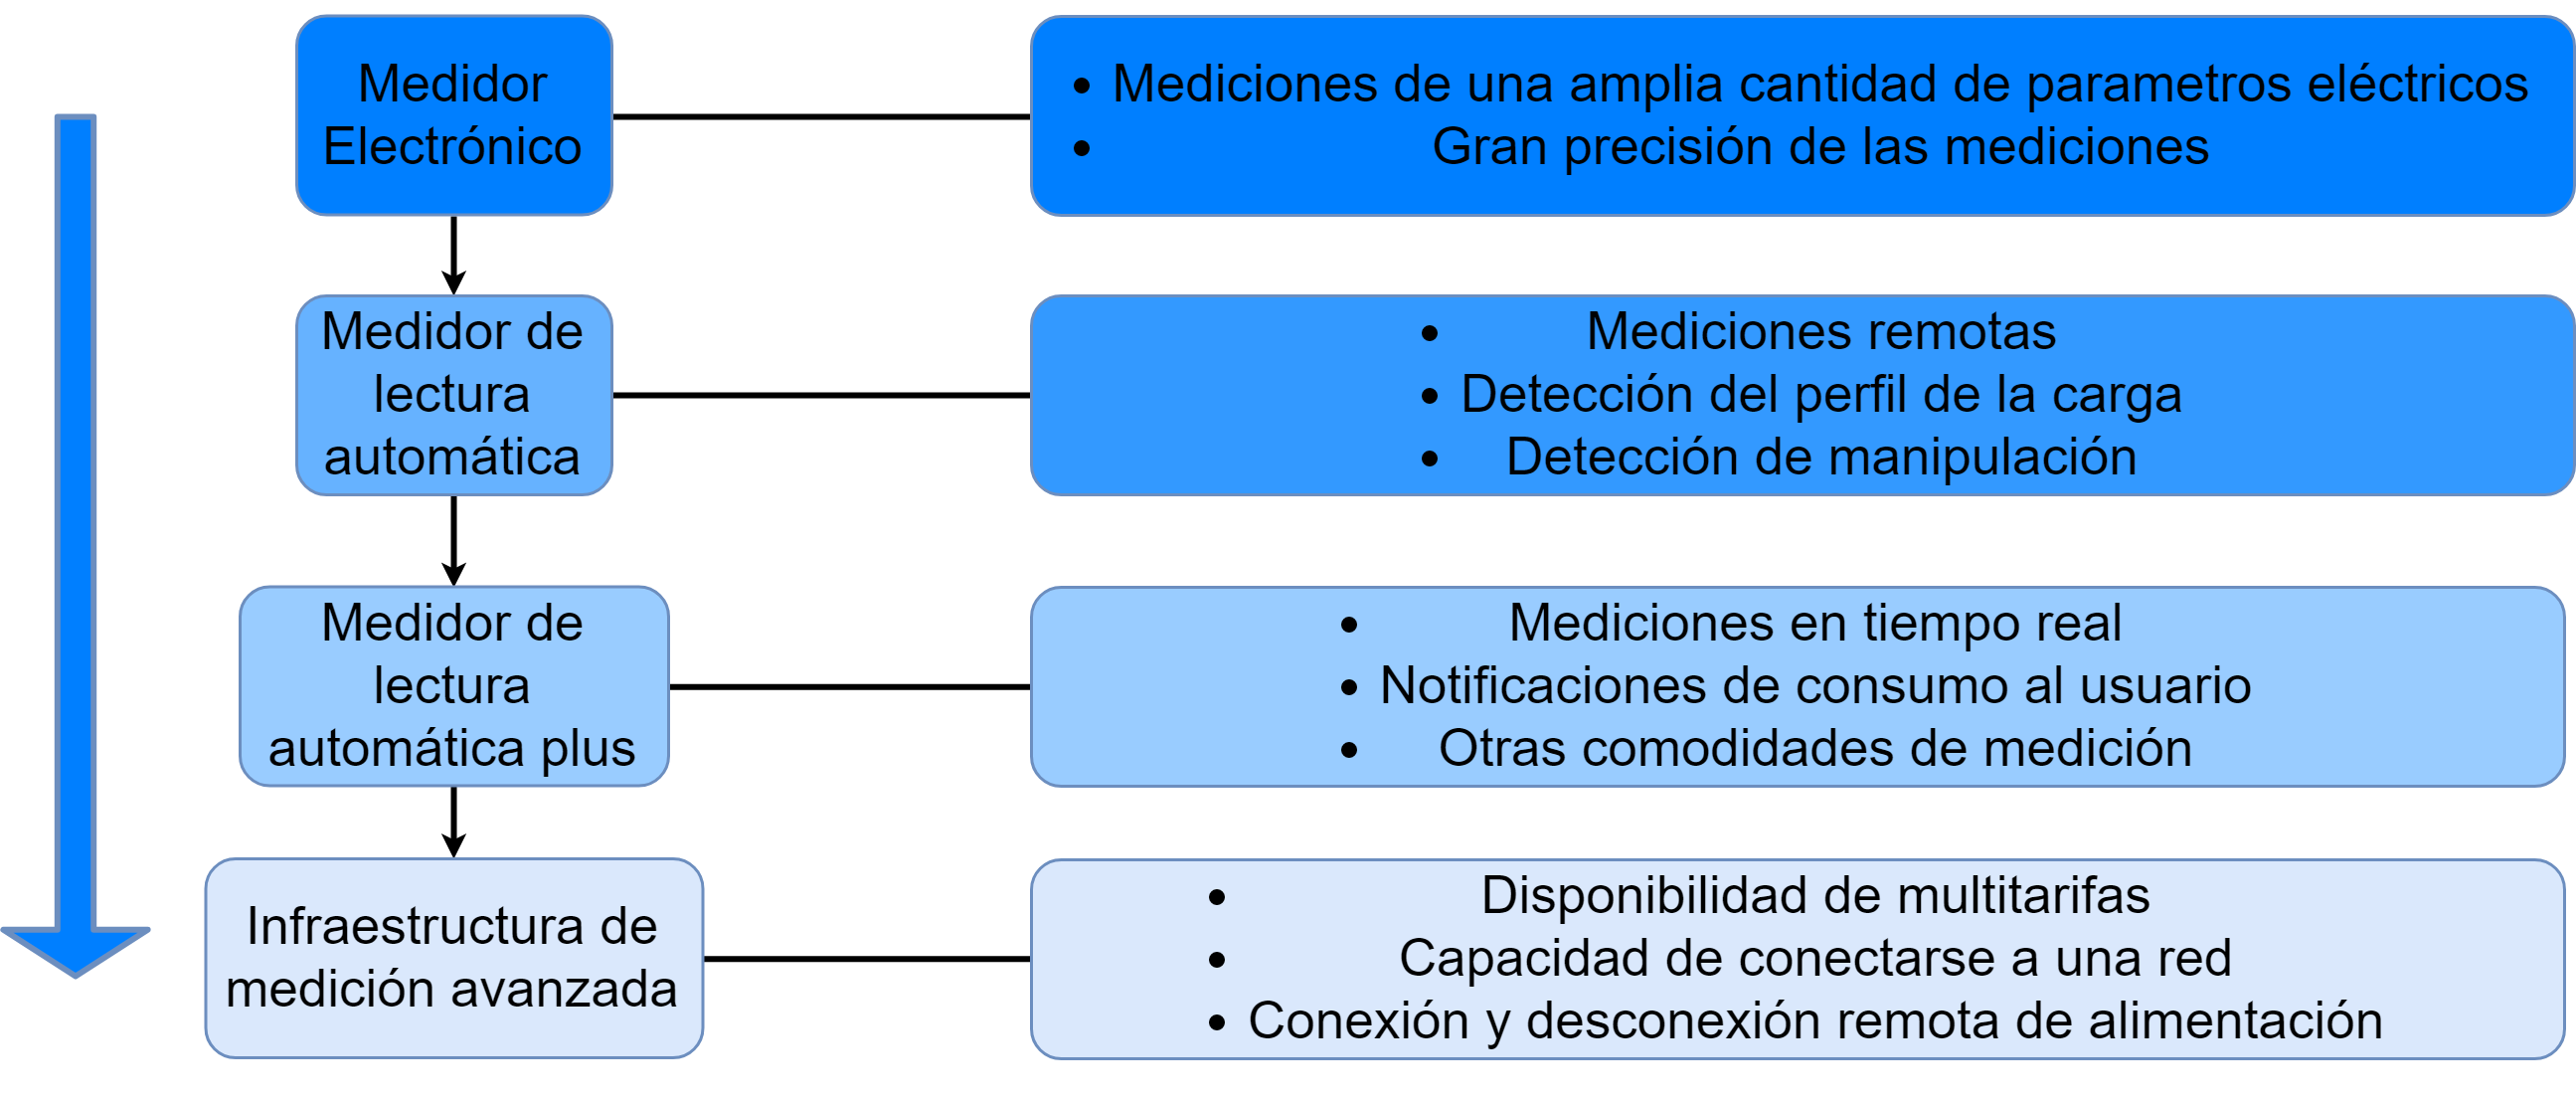
\includegraphics[width=0.8\textwidth]{../Imagenes/Evolucion_medidores.png}
    \caption{Evolución de los medidores de consumo eléctrico}
    \label{fig:Evol_MI}
  \end{figure}

  \par A pesar de la evolución de estos dispositivos


  \subsection{Características}

  \subsection{Estandarización}

  \subsection{Estructura}
    \subsubsection{Sensado}
    \subsubsection{Acondicionamiento}
      \par Existen maneras de cuantificar un fenómeno físico con parámetros eléctricos
      mediante la utilización de sensores electrónicos, sin embargo, la salida de estos
      no siempre es apta para realizar un procesamiento de la data, por lo que es necesario
      acondicionar la señal adquirida mayormente mediante distintos circuitos eléctronicos
      que ofrecen funciones como: ajuste de ganancia y nivel, filtrado, adaptación de impedancia
      y aislamiento.


      \subsubsubsection{Ajuste de ganancia y nivel}
      \par En busca de lograr una amplificación o una atenuación es necesario conocer
      los amplificadores operacionales (OPAM), estos dispositivos electrónicos son capaces
      de alterar la señal electrica en su entrada, multiplicando su valor por una ganancia
      determinda por la configuración externa. Por ejemplo, la configuracion no-inversora:

      (IMAGEN DE LA CONFIGURACION NO INVERSORA)

      \par Logrando transformar una señal que oscila entre -10 y +10 V a una entre -2.5 y 2.5 V, estableciendo una ganancia de 0.25.

      \par Por otro lado comunmente los dispositivos electrónicos no son capaces de procesar
      señales bipolares, por lo tanto se debe hacer un ajuste del nivel a las señales bipolares.
      Este ajuste se puede lograr mediante la utilización de un divisor de tensión resistivo
      mostrada a continuación:

      (IMAGEN DE LA CONFIGURACION DEL AJUSTE DE NIVEL)

      \par Con esta configuración es posible llevar una señal eléctrica oscilante entre -2.5 y 2.5 V a una entre 0 y 5 V.

      \subsubsubsection{Filtrado}
      \subsubsubsection{Adaptación de impedancia}
      \subsubsubsection{Aislamiento}
      \par Por motivos de seguridad es necesario separar

    \subsubsection{Conversion}
      \par Es necesario digitalizar las señales eléctricas de tal modo que el dispositivo de procesamiento sea capaz de interpretar y hacer el procesamiento de estas. La digitalización de señales es dependiente de las caracteristicas de la señal a adquirir y de los conversores de señales analógicas a digitales o como se conocen por sus siglas en ingles ADC (\textit{Analog to Digital Converter"}).

      \subsubsubsection{Teorema de muestreo Nyquist-Shannon}
        \par Las señales eléctricas poseen características como amplitud, forma, frecuencia, entre otras. Para la recreación exacta de las señales periódicas se requieren una cantidad de muestras necesarias. El teorema de Nyquist-Shannon considerado uno de los mas importantes en la teoría de adquisición establece que se necesita una frecuencia de muestreo de al menos el doble de la frecuencia de la señal a adquirir.
        \begin{equation}
          F_s \geq 2*F_m
        \end{equation}
        \subsubsubsection{Conversor analógico-digital}
          \par Los conversores se encargan de representar las señales analógicas con valores binários por medio de diferentes circuitos electróonicos.
          \begin{itemize}
            \item Muestreo: como establece el teorema de Nyquist-Shannon la frecuencia de muestreo establecera cada cuanto se debe tomar una muestra de la señal analógica para la recreación exacta de esta en el mundo digital.
            \item Cuantificación: en la mayoria de los casos los valores analógicos poseen minimas variaciones que no pueden ser represantadas mediante el bit menos significativo, es por esto que es necesario realizar una aproximación de los valores de la señal analógica.
            \begin{figure}[H]
              \centering
              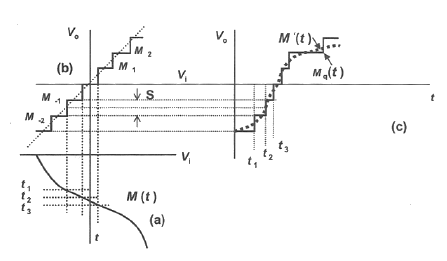
\includegraphics[width=0.6\textwidth]{../Imagenes/Cuantificacion.png}
              \caption{Convertidor analógico digital de aproximaciones sucesivas (REFERENCIA)}
              \label{fig:Cuantificacion}
            \end{figure}
            \item Conversores digitales a analógicos: al contrario de los conversores analógicos digitales estos se encargar de transformar señales digitales en analógicas mediante comparadores y acoplamientos de resistencias que permitan generar distintos voltajes en su salida.
          \end{itemize}

          \par Los dispositivos evaluados para la realización del medidor poseen un ADC de aproximaciones sucesivas y este se encuentra estructurado por un convertidor digital a analógico, un comparador analógico y un circuito de control.

          \begin{figure}[H]
            \centering
            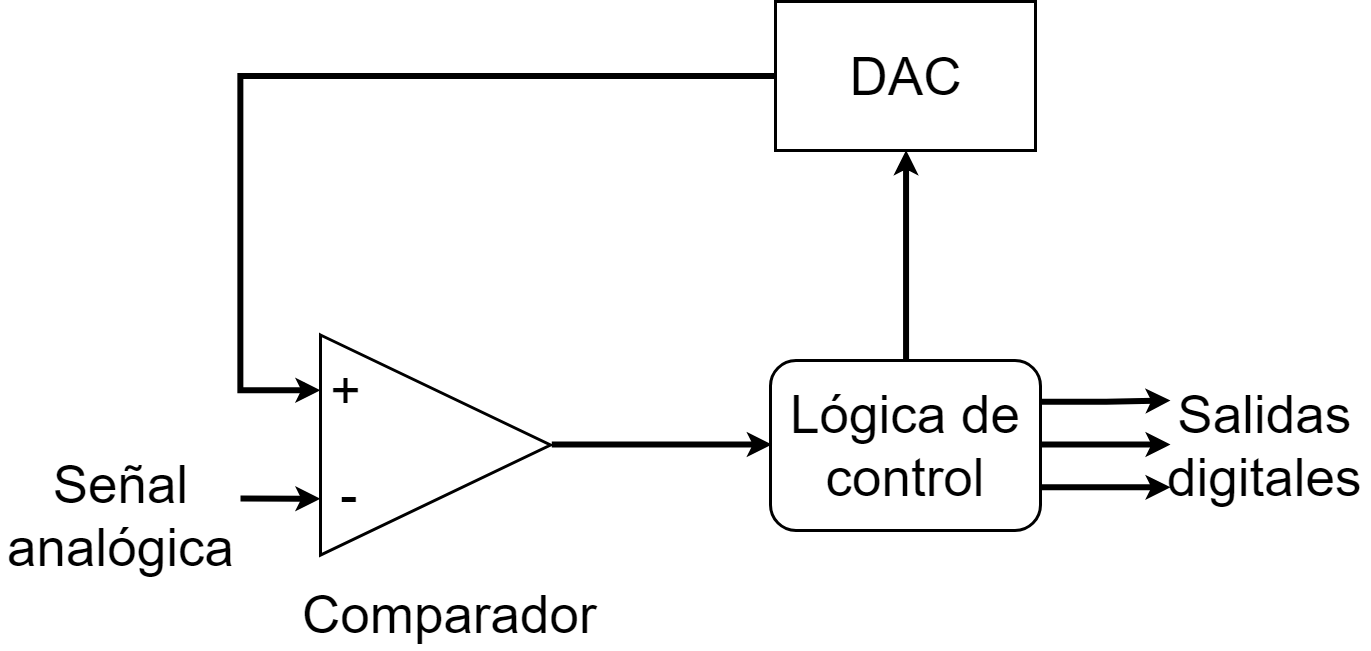
\includegraphics[width=0.5\textwidth]{../Imagenes/ADC.png}
            \caption{Convertidor analógico digital de aproximaciones sucesivas}
            \label{fig:ADC_aproximaciones_sucesivas}
          \end{figure}

          \par El principio de funcionamiento de este ADC es el siguiente:
          \begin{enumerate}
            \item El controlador asigna un 1 al bit mas significativo del DAC, dejando el resto de los bits en 0.
            \item Se compara la señal analógica a muestrear con el valor del DAC, si este es menor se convierte el bit a 0 y se coloca el siguiente bit menos significativo a 1.
            \item Se repite el proceso 1 y 2 hasta cubrir todos los bits del DAC.
          \end{enumerate}

          \par En la figura (REFERENCIA) podemos observar un ejemplo de como la señal de salida del DAC se aproxima al valor de referecia en fracciones de la frecuencia de muestreo.

          \begin{figure}[H]
            \centering
            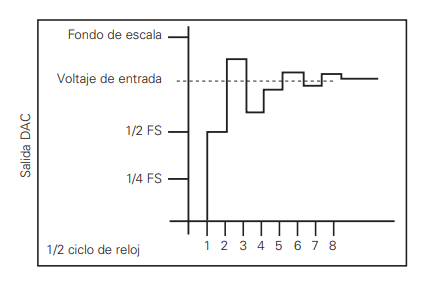
\includegraphics[width=0.5\textwidth]{../Imagenes/ADC_ejemplo.png}
            \caption{Salida del DAC del conversor analógico digital (REFERENCIA)}
            \label{fig:ADC_DAC_ejemplo}
          \end{figure}


    \subsubsection{Procesamiento}
      \subsubsubsection{Valores efectivos}

      \subsubsubsection{Potencia}
      \begin{itemize}
        \item Aparente
        \item Activa
        \item Reactiva
      \end{itemize}

      \subsubsubsection{Factor de potencia}

      \subsubsubsection{Distorsión armónica}

      \subsubsubsection{Distorsión armónica}
      \subsubsubsection{Energia}
    \subsubsection{Comunicación}
      \subsubsubsection{Serial}
      \subsubsubsection{DLSM/COSEM}
      \subsubsubsection{Modbus}

\section{Labview}
  \subsection{Dispositivos Real-Time}
  \subsection{Algoritmos utilizados}
